\chapter{General expectations}
\label{ch:expectations}
\index{expectations}

\section{First week of teaching}
\tfaq[1]{0mm}{What should I be doing in the first week of teaching?}{General~questions}
\index{expectations!first~week~of~teaching}
As a coursework only module, you need to dedicate a substantial amount of time to the \ac{SEG} during term time.  The module has been designed to ensure you can dedicate as much time as you want early on in the module, so there is no excuse to delay your engagement with the module. In fact, early engagement with the module is crucial.

\begin{figure}
\checkoddpage \ifoddpage \forcerectofloat \else \forceversofloat \fi
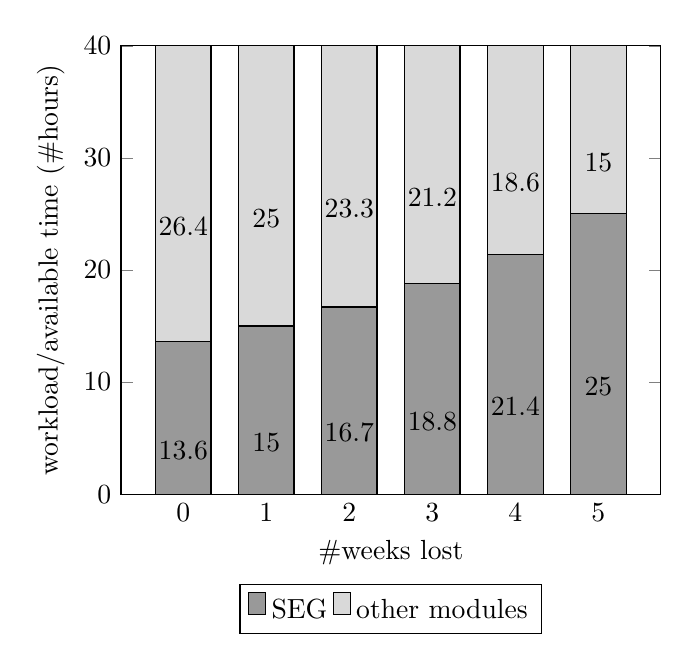
\begin{tikzpicture}
\begin{axis}[
    ybar stacked,
    nodes near coords,
    every node near coord/.append style={yshift=-5pt,anchor=north},
    bar width=20pt,
    ymin=0,
    ymax=40,
    enlarge x limits=0.15,
    legend style={at={(0.5,-0.2)},
      anchor=north,legend columns=-1},
    xlabel={\#weeks lost},
    ylabel={workload/available time (\#hours)},
    symbolic x coords={0,1,2,3,4,5},
    xtick=data,
    ]
\addplot+[ybar,black,fill=gray!80,text=black] plot coordinates {(0,13.6) (1,15) (2,16.7) (3,18.8) (4, 21.4) (5, 25)};
\addplot+[ybar,black,fill=gray!30,text=black] plot coordinates {(0,26.4) (1,25) (2,23.3) (3,21.2) (4, 18.6) (5, 15)};
\legend{\strut \ac{SEG}, \strut other modules}
\end{axis}
\end{tikzpicture}
\caption{\ac{SEG} workload and time available to work on other modules (expressed in \#hours) in relation to the number of weeks no work is done for this module.}
\label{fig:workload-to-weeks-lost}
\end{figure}

Figure~\ref{fig:workload-to-weeks-lost} plots the weekly workload for this module relative the number of weeks you do not or cannot engage with it.    As you can see, the \ac{SEG} workload increases substantially as engagement with it is delayed.  Figure~\ref{fig:workload-to-weeks-lost}  also shows the amount of time left to work on other modules, assuming a 40 hour work week.  Bear in mind that, in Year 2, you have another coursework-only module with similar workload requirements to this one. The time available for that and other modules diminishes quickly.

\newthought{In the first week of teaching}, you should aim to achieve the following:
\begin{itemize}
\item Ensure you have access to a development environment with a UNIX command-line interface, Python 3 with pip, and git.  This is a means to start learning Python and Django, so do not waste too much time on this.  If you find it very difficult to install this software on your desktop or laptop PC, use a Faculty lab machine or student VM, rather than postponing engagement with the course.
\item Learn all or most of the Python course, completing the exercises as you encounter them.
\item Complete the version control for individuals course.
\item Attend the first lecture.
\end{itemize}



\section{Independent study}
\tfaq[1]{0mm}{What is the ``independent study'' component of the module?}{General~questions}
\index{expectations!independent~study}
In Semester 1, you will be learning to program in Python and develop web application with Django, which is a framework developed in Python.  You will also learn to use certain tools that support web development, including tools for build automation, automated testing, version control, and deployment of web applications.  These topics require you to develop new practical knowledge and skills.  The amount of new theoretical or conceptual content, beyond what you already learned in Year 1, is limited.  

In my view, such content is best learned outside of lecture theatre.  One effective approach is to learn content in small bursts, followed immediately by exercises.  Another is to follow along with a demonstration on your own computer, mimicking each step that is demonstrated.  In this module, you will be using both these approaches to learn Python, Django, and a range of devops tools.  There will be some forms of support to help you out when you get stuck, but you should be going through this material as independently as you can.  

In your independent study, consider the following:
\begin{itemize}
\item In the first five weeks of Semester 1, before the group project start, you should dedicate a substantial majority of your weekly study time for this module (approximately 15hrs/week) to independent study.  Do not postpone this as it will be hard to catch up later.
\item \emph{Complete all exercises}.  When shown demonstrations, replicate each demonstration on your workstation.  The independent study material is very practical and merely watching the videos is not sufficient to learn it.
\item Encountering \emph{bugs, errors, and unwanted exceptions} are an important part of the learning process.  It can be frustrating to lose hours on attempts to overcome such problems.  But don't consider them a waste of time.  Resolving bugs when attempting to replicate a demonstration or solving exercises helps you identify and overcome misconceptions.  It also also develops your debugging skills.
\item Work through the material at your own pace.  Speeding through material you do not already know in a misguided attempt to get ahead will make the later material harder to digest.  \emph{Everyone learns certain material at a different pace}.  Allow yourself to set the pace that works for you.  Of course, a timely start with independent learning helps.
\item All independent study material is labelled as ``Core'', ``Recommended'', or ``Optional''.\index{independent~study}  You need to complete the ``Core'' material before reading week in Semester 1 as it covers the essential knowledge and skills required to participate in the small group project.  Knowledge and skills covered by the ``Recommended'' is referred to in some of the small group project marking criteria for 60-70\%.  Learn this only after you completed all ``Core'' material.  The ``Optional'' material concerns more advanced, niche topics.  You will need to be more independent to study this material.  The ``Optional'' material is referenced in some of the small group project marking criteria for 80\% and higher.
\end{itemize}

Software Engineering is a rapidly evolving field.  New languages, frameworks, and tools are introduced regularly.  Existing ones change all the time.  As a software engineer, you will need to stay up-to-date with these developments.  Therefore, it is important that you develop the skillset needed to learn new technology independently.  The independent study materials develop these skills.

\section{Tutorials}
\tfaq[1]{0mm}{What is the roles of large and small group tutorials?  Do they cover different material from the independent study component?}{General~questions}
\index{expectations!large~group~tutorials}
\index{expectations!small~group~tutorials}
Along with the independent study component, Semester 1 large and small group tutorials seek to prepare you for group project work.  Beware that the independent study component, the large group tutorial, and small group tutorials serve different purposes and cover different material!  You will need to engage with all these activities as one does not substitute another.

The \emph{small group tutorials}\index{small~group~tutorials} aim to develop your practical skillset to manage, and participate constructively with fellow team members software engineering group projects.  The activities are designed to put key elements of the software engineering and project management training videos into practice.  it is advisable to engage with both concurrently.

The \emph{large group tutorials}\index{large~group~tutorials} aim to complement all independent learning activities: Python/Django training, devops training, and software engineering and project management training.  A session will consist of quizzes designed to identify potential misconceptions, a class discussion around project management case studies, and a Q\&A activity.

\subsection{Small group tutorials}
\tfaq[1]{0mm}{What will I learn in the small group tutorials?}{General~questions}
\index{expectations!small~group~tutorials}
Each small group tutorial starts with an informal icebreaker activity.  This is intended to put everyone at ease before discussing certain topics in break-out groups.  It also offers an opportunity to get to know the classmates in your tutorial group a bit better.  Getting to know others is an important networking skill that will help you find team mates for the major group project.

A significant portion of each group project is dedicated to discussion, negotiation, and peer review in small break out groups.  In these break-out groups, you will learn the most important skills and activities needed to coordinate work with teammates.  The small group tutorial sessions include the following activities:
\begin{itemize}
\item Agreeing a \emph{team charter}\index{team~charter} within a small group.
\item Performing a \emph{code review}\index{code~review}.
\item Estimating effort in a group through planning poker.
\item \emph{Risk management}index{risk~management}:Identifying, analysing, and planning for uncertainty and risk.
\item \emph{Agile planning}{planning!agile}: Writing user stories, specifying a Kanban board process, and managing the development of a consistent user interface.
\end{itemize}

The end of each session includes a class discussion to reflect on how well the activity went and what you learned (e.g. what you would do again or what you would do differently).

\subsection{Large group tutorials}
\tfaq[1]{0mm}{What will I learn in the large group tutorials?}{General~questions}
\index{expectations!large~group~tutorials}
As the large group tutorials aim to complement the independent learning/training videos, there is some flexibility as to what is covered.  Your feedback will be considered and can lead to a change in plans, though I will also take into account what students in previous years needed support with throughout the module.

A typical session consists of four parts:
\begin{itemize}
\item \emph{Announcements/guidance}: In this part, I will share important information with you.  This information may include issues people have struggled with, changes to the information on KEATS, responses to feedback I received from you, and reminders of important information you should be aware of.
\item \emph{Quizzes/exercises}: The quizzes and exercises cover (mostly technical) Python, Django, and devops challenges based on misconceptions students and teams have faced in the past.  The purpose of these exercises is to resolve and avoid these misconceptions, to that it will be easier for you to learn.
\item \emph{Class conversations}: The class conversations cover project management challenges based questions and challenges group project teams have faced in previous years.  You will be encourage to think about certain problems and share your opinions.  These conversations are not intended to be debates.  They are not intended to be ``won'' by any side.  While I will share my views at the end of each class conversation, you are entitled to your own opinions.  I hope that these conversations will help you learn to think in more nuanced terms about project management and leadership challenges. 
\item \emph{Q\&A}: Each session will conclude with some time for Q\&A.  Before each session, the large group tutorial section hosts a forum where you can upvote questions of others, or propose your own questions.  The forum closes at 5pm the day before the session.  The most upvoted questions will be prioritised in the session.
\end{itemize}

\section{Working in groups}
\index{expectations!group~work}
\subsection{Core expectations}
\tfaq[1]{0mm}{What is expected of me in the group projects?}{General~questions}
\marginnote{\vspace{0mm}\newthought{Further reading}: Each group project comes with its own handbook, which you should read as you are participating in these projects.  You find them on KEATS in \emph{Small group project $\rightarrow$ Handbook: Small group project} and \emph{Major group project $\rightarrow$ Handbook: Major group project} respectively.}
As explained earlier, the small and major group projects differ in scale and purpose.  Consequently, each comes with its own set of expectations.  Nevertheless, there is a core set of expectations for both group projects and it is crucial that you meet them.  The expectations listed below are fundamental though, so you should adhere to them and expect you team mates to adhere to them.
\begin{itemize}
\item In the group projects, you will be working closely with fellow students.  You are expected to \emph{behave respectfully} to one another during lectures, outside of lectures, in meetings, when communicating online, through email, or through collaborative development tools.  The College does not tolerate inappropriate or demeaning comments related to gender, gender identity and expression, sexual orientation, disability, physical appearance, race, religion, age, or any other personal characteristic.  If you witness or experience any behaviour you are concerned about, please speak to someone about it.
\item Group work requires \emph{communication} and \emph{coordination}.  As a team, you must agree project objectives, plan and schedule work towards those objectives, monitor progress, and agree remedial actions when plans/schedules fail or other problems arise.  Individual members of the team cannot do whatever they want: work on the tasks you you have been assigned and \emph{only} on tasks you have been assigned.  \emph{Regular, minuted, whole-team meetings} are the primary method of communication and coordination. 
\item Team members must make every effort to \emph{attend all meetings, on-time, from start to finish}.  Engage actively with the meetings by adopting \emph{all} of the following: listen to others, sharing your views, volunteer to take on tasks you are able to do, show the work that you have done, read the meeting minutes following the meeting, and report any errors.  Your team mates are not your personal assistant: do not expect your team mates to keep track of team decisions or your responsibilities for you.  You need to do that yourself.
\item Every member of the team must make a meaningful contribution to the team's code base every week of the software build period.  That implies nobody is excused from coding!  A \emph{week} is defined as period from Monday to Sunday (inclusive).  The project's \emph{software build  period} corresponds to the weeks in which at least some team members are writing code.  In the small group project, the software build  period should encompass the full six weeks of the project.  In the major group project, it is likely to be a little less than the full ten week period of the project because of the amount of non-coding work involved.
\end{itemize}

%%% Restructure this section...



\section{Feedback and peer assessments}
\label{sect:feedback-and-peer-assessments}
\tfaq[1]{0mm}{How should give feedback to/write peer assessment for my teammmates?}{General~questions}
\index{peer~assessments!expectations}
As this is a module is about working with others, you will have to tell others how they are doing or how they did.  

You will participate in two peer assessment exercises (via Team Feedback)\index{peer~assessments!Team Feedback}\index{Team Feedback!peer~assessments}, one after each group project.  In a peer assessment exercise, you are required to fill out a form for each of your team member: including a number of multiple choice questions and a feedback field.   \emph{The feedback text is a critical component of any peer assessment.}  Without any feedback text, a peer assessment will not be awarded any marks.  At the very least, explain why you scored your team mate in the way that you did in the multiple-choice section.  Without any feedback, the peer review is merely a collection of vague claims.  You can also use the feedback field to elaborate on your experiences with a team member, provide some detail and context for your review, illustrate claims with some examples or anecdotes, and reflect what you or your team might have learned in group project exercise.

If there is good communication within your team, the feedback in peer assessments should not come as a surprise.  Team members should talk to each other about how the project is going.  Concerns should be shared within the team: ideally at team meetings if it concerns everyone, or at a one-to-one meeting if a difficult conversation with a single person is required.

When you write feedback, \emph{be considerate and inclusive}.  Another fellow human being will hear what you are saying or read what you have written.  Disparaging criticism without nuance or consideration of the reviewee can be hurtful -- ultimately, it is counter productive.  That does not mean your feedback should be relentlessly positive or minimise valid criticism.  On the contrary, it is important to voice genuine concerns in a \emph{timely} manner, and persistently follow it up.  Peer assessments should contain an \emph{accurate and complete critique}: do not gloss over the problem.  

There are some techniques you can employ to formulate negative feedback considerately and \emph{constructively}.  Examples include, but are not limited to the following.
\index{feedback!giving~negative}
\begin{itemize}
\item \emph{Balance negatives with specific, meaningful praise}.  Criticism in feedback tends to be more acceptable to the recipient if the feedback also incorporates due recognition to positive experience.  Be specific (not vague) when praising your peer in feedback to show you paid attention and appreciated what went well.  Make sure that the praise concerns meaningful issues.  Faint praise can come across as condescending, or even as criticism in disguise.  Praise is only a usable tool if you have something of value to complement.
\item You can take the previous method one step further with \emph{the sandwich method}.  In the sandwich method, you start by saying something positive about the other person, then introduce the negative feedback, and conclude with more positive feedback.  This can work especially when you need to give negative feedback to someone in person.  People do tend to recognise the sandwich method, so it is especially important that any positive feedback you want to use here is genuine.
\item In your feedback, \emph{focus on actions and behaviours}.  Talk about facts, such as commitments made, deadlines missed, GitHub activity, meeting attendance.  Our actions and behaviours are not necessarily representatives of our personality and character.  We can change our actions and behaviours.  It is harder to change our personality or character.  If feedback concerns the person, rather than their actions and behaviours, then it becomes something that is difficult to correct or address.
\item \emph{Use sentences start with ``I''}, such as ``I think [...]'' or ``I feel [...]''.  By starting a sentence with ``I'', you are forcing yourself to focus on your perceptions and views of the other person's actions and behaviours.  It is another way to avoid making the negative feedback about the person being criticises.
\item Always ensure your negative feed back is \emph{specific}.  Vague feedback tends to be very demoralising.  On the one hand, it suggests concerns are broader than they really are.  On the other hand, vague feedback is hard to act on.
\item \emph{Provide actionable feedback}.  This gives your peer agency and control over a problem, as well as an opportunity to address it.
\end{itemize}

\index{feedback!positive~reinforcement}
Negative feedback is not the only tool in your arsenal to encourage your team mates to do the right thing.  Negative feedback's counterpart -- \emph{positive reinforcement} -- can be more effective if you make a point of praising people consistently and regularly for what they do well.